\documentclass[article]{jss}
\usepackage{rotating}
\usepackage{pdfpages}
\usepackage{booktabs}
\usepackage{setspace}
\usepackage{lscape}
\usepackage{natbib}

\author{Garrett Grolemund\\Rice University \And 
        Hadley Wickham\\Rice University}
\title{Dates and Times Made Easy with \pkg{lubridate}}

\Plainauthor{Garrett Grolemund, Hadley Wickham}
\Plaintitle{Dates and times made easy with lubridate}
\Keywords{dates, times, time zones, daylight savings time, \proglang{R}}
\Plainkeywords{dates, times, time zones, daylight savings time,  R}

%% publication information
%% \Volume{13}
%% \Issue{9}
%% \Month{September}
%% \Year{2004}
%% \Submitdate{2004-09-29}
%% \Acceptdate{2004-09-29}

\Address{
  Garrett Grolemund\\
  Rice University\\
  Houston, TX 77251-1892, United States of America\\
  E-mail: \email{grolemund@rice.edu}
}

\Abstract{
  This paper presents the lubridate package for \proglang{R} \citep{R}, which facilitates working with dates and times.  Date-times create various technical problems for the data analyst. The paper highlights these problems and offers practical advice on how to solve them using \pkg{lubridate}.  The paper also introduces a conceptual framework for doing math with date-times.
}

%\setstretch{2}
\begin{document}

\section{Introduction}

Date-time data can be frustrating to work with. It comes in many different formats, which makes recognizing and parsing it a challenge. Will our program handle the format that we have? If it does, we still face a slew of problems specific to date-times. How can we easily extract components of the date-times, such as years, months, or seconds? How can we switch between time zones, or compare times from places that use daylight savings time (DST) with times from places that do not? Date-times create even more complications when we try to do math with them. Conventions such as leap years and DST make it unclear what we mean by ``one day from now" or ``exactly two years away."  Even leap seconds can disrupt a seemingly straight forward calculation.  This complexity affects other tasks too, such as constructing sensible tick marks for plotting date-time data.

While base \proglang{R} \citep{R} handles some of these problems, the syntax it uses is uninviting, often confusing, and difficult to remember. Moreover, the correct \proglang{R} code often changes depending on the class of date-time object being used. \pkg{lubridate} acknowledges these problems and makes it easier to work with date-time data in \proglang{R}. Specifically, \pkg{lubridate} helps users:

\begin{itemize}
   \item Identify and parse date-time data, Section~\ref{sec:parsing}.
   
    \item Extract and modify components of a date-time, such as years, months, days, hours, minutes, and seconds, Section~\ref{sec:accessors}.
  
  \item Perform accurate math on date-times, Section~\ref{sec:types}.
    
  \item Handle time zones and Daylight Savings Time, Sections~\ref{sec:tz}, and~\ref{sec:DST}.
  
\end{itemize}

\pkg{lubridate} uses an intuitive user interface inspired by the date libraries of object oriented programming languages.  \pkg{lubridate} methods are compatible with a wide-range of common date-time objects. These include character strings, POSIXct, POSIXlt, Date, chron ~\citep{chron}, fCalendar ~\citep{fCalendar}, zoo ~\citep{zoo}, xts ~\citep{xts}, its ~\citep{its}, tis ~\citep{tis}, timeSeries ~\citep{timeSeries}, fts ~\citep{fts}, and tseries ~\citep{tseries} objects. Note that \pkg{lubridate} overrides the + and - methods for POSIXt, Date, and difftime objects in base \proglang{R}.

The time concepts introduced by \pkg{lubridate} are inspired by the \proglang{Java} based JODA time project \citep{jodatime}. This paper demonstrates the convenient tools provided in the \pkg{lubridate} package and ends with a case study, which uses \pkg{lubridate} in a real life example.

This paper describes \pkg{lubridate} 0.1, which can be downloaded from {\sc cran}. Development versions can be found at \url{http://github.com/hadley/lubridate}.

\section{Motivation}

To see how \pkg{lubridate} simplifies things, consider a common scenario. We have a character string. We'd like to read it in as a date-time, extract the month, and change it to February (i.e. 2). On the left are the base \proglang{R} methods we'd use for these three tasks.  On the right are the \pkg{lubridate} methods.

\begin{center}
  \begin{tabular}{|p{7cm}|p{7cm}|}
    \hline
    \proglang{base R} & \pkg{lubridate}\\
    \hline
    \code{date <- as.POSIXct("01-01-2010", } & \code{date <- dmy("01-01-2010")}\\
    \indent \code{   format = "\%d-\%m-\%Y", tz = "UTC")} & \\
    & \\
    \code{as.numeric(format(date, "\%m"))} \# or  & \code{month(date)}\\
   \code{as.POSIXlt(date)$month + 1} &\\
    & \\
     \code{date <- as.POSIXct(format(date, } & \code{month(date) <- 2} \\
 \indent \code{   "\%Y-2-\%d"))} & \\
 \hline
\end{tabular}
\end{center}

Now we'll go a step further. We'll go back a day in time and display our new date in the Greenwich Meridian time zone (GMT).

\begin{center}
  \begin{tabular}{|p{7cm}|p{7cm}|}
    \hline
     \proglang{base R} & \pkg{lubridate}\\
    \hline
    \code{seq(date, length = 2, by =}  & \code{date - days(1)} \\
    \indent \code{   "-1 day")[2]} & \\
   & \\
   \code{as.POSIXct(format(as.POSIXct(date),}  & \code{with_tz(date, "GMT")}\\
  \indent \code{    tz = "UTC"), tz = "GMT")} &\\
    \hline
\end{tabular}
\end{center}

\pkg{lubridate} makes basic date-time manipulations much more straight forward. Plus, the same \pkg{lubridate} methods work for all of the popular date-time object classes (\code{Date}, \code{POSIXt}, \code{chron} ...).

Figure~\ref{fig:comparison} provides a more complete comparison between \pkg{lubridate} methods and base \proglang{R} methods. It shows how \pkg{lubridate} can simplify each of the common date time tasks presented in RNews Volume 4/1, June 2004 \citep{Rnews}. It also provides a useful summary of \pkg{lubridate} methods.
% Always a good idea to show some examples right off the bat.  This helps
% people understand why they should bother reading the paper

\begin{figure}[htpb]
  \includegraphics[angle=90, scale = 2]{comparison-table}

%  \caption[angle=90]{\pkg{lubridate} comparison (adapted from R News Volume 4/1, June 2004)} 
  \clearpage

  \label{fig:comparison}

\end{figure}





\section{Parsing date-times}
\label{sec:parsing}

We can read dates into R using the \code{ymd()} series of functions provided by \pkg{lubridate}. The letters y, m, and d correspond to the year, month, and day elements of a date-time. To read in a date, choose the function name that matches the order of elements in your date-time object. For example,\\

\code{R> mdy("12-01-2010")}\\
\code{[1] "2010-12-01 UTC"}\\

or

\code{R> dmy("12-01-2010")}\\
\code{[1] "2010-01-12 UTC"}\\

or

\code{R> dmy(c("31.12.2010", "01.01.2011"))}\\
\code{[1] "2010-12-31 UTC" "2011-01-01 UTC"}\\


These functions create a POSIXct date-time object that matches the date described by the character string.  The functions automatically recognize the following separators: ``-", ``/", ``.", and ``" (i.e., no separator). When a \code{ymd()} function is applied to a vector of dates, \pkg{lubridate} will assume that all of the dates have the same order and the same separators. It will also print a message that tells the user which format was used to parse the dates. \code{ymd()} type functions also exist for times recorded with hours, minutes, and seconds. These functions make it simple to parse any date-time object that can be converted to a character string. See Table~\ref{tbl:parsers} for a complete list of \code{ymd()} type parsing functions. 

\begin{table}
  \begin{center}
  \begin{tabular}{ll}
  \toprule
  Order of elements in date-time & Parse function\\
  \midrule
  year, month, day & \code{ymd}\\
  year, day, month  & \code{ydm}\\
  month, day, year & \code{mdy}\\
  day, month, year & \code{dmy}\\
  hour, minute & \code{hm}\\
  hour, minute, second & \code{hms}\\
  year, month, day, hour, minute, second & \code{ymd.hms}\\
  \bottomrule
    
  \end{tabular}
  \end{center}
  \caption{Parse functions based on order of date-time elements.}
  \label{tbl:parsers}
\end{table}

\section{Manipulating date-times} 
\label{sec:accessors}

Every date-time is a combination of different elements, each with its own value. For example, most date-times include a year value, a month value, a day value, etc. Together, these elements specify the exact moment that the date-time refers to. We can easily extract each element of a date-time with the accessor function that has its name, as shown in Table~\ref{tbl:accessors}. For example,  if we save the current system time\\

\code{R> date <- now()}\\
\code{[1] "2010-02-25 09:51:48 CST"}\\

we can extract each of its elements.\\

\code{R> year(date)}\\
\code{[1] 2010}\\

\code{R> minute(date)}\\
\code{[1]  51}\\

For the month and weekday elements (wday), we can also specify whether we want to extract the numerical value of the element, an abbreviation of the name of the month or weekday, or the full name. For example,

\code{R> month(date)}\\
\code{[1] 2}\\

\code{R> month(date, label = TRUE)}\\
\code{[1] Feb}\\

\code{R> month(date, label = TRUE, abbr = FALSE)}\\
\code{[1] February}\\

\code{R> wday(date, label = TRUE, abbr = FALSE)}\\
\code{[1] Thursday}\\

\begin{table}
  \begin{center}
  \begin{tabular}{ll}
  \toprule
  Date component & Accessor\\
  \midrule
  Year & \code{year()}\\
  Month & \code{month()} \\
  Week  &\code{week()} \\
  Day of year & \code{yday()} \\
  Day of month & \code{mday()}\\
  Day of week & \code{wday()}\\
  Hour & \code{hour()}\\
  Minute & \code{minute()}\\
  Second & \code{second()}\\
  Time Zone & \code{tz()}\\
  \bottomrule
    
  \end{tabular}
  \end{center}
  \caption{Date-time accessors used by lubridate.}
  \label{tbl:accessors}
\end{table}

We can also use any of the accessor functions to set the value of an element. This would also change the moment that the date-time refers to. For example,\\

\code{R> day(date) <- 5}\\
\code{[1] "2010-02-05 09:51:48 CST"}\\

changes our date to the fifth day of the month. We can also set the elements to more complicated values, e.g.\\

\code{R> minute(dates) <- mean(minute(dates))}\\

Note that if we set an element to a larger value than it supports, the difference will roll over into the next higher element. For example,\\

\code{R> day(date) <- 30}\\
\code{[1] "2010-03-02 09:51:48 CST"}\\

We can use this to find the last day of a month:\\

\code{R> day(date) <- 1}\\
\code{R> month(date) <- month(date) + 1}\\
\code{R> day(date) <- day(date) - 1}\\
\code{[1] "2010-03-31 09:51:48 CDT"}\\


Lubridate also provides an update method for date-times.  This is useful if you want to change multiple attributes at once or would like to create a modified copy, instead of transforming in place.\\

\code{R> update(date, year = 2010, month = 1, day = 1)}\\
\code{[1] "2010-01-01 09:51:48 CST"}\\

Finally, we can also change dates by adding or subtracting units of time from them. For example, the methods below produce the same result.\\

\code{R> hour(date) <-  12 }\\
\code{[1] "2010-02-25 12:51:48 CST"}

\code{R> date + hours(3) }\\
\code{[1] "2010-02-25 12:51:48 CST"}\\

Notice that \code{hours()} (plural) is not the same function as \code{hour()} (singular). \code{hours()} creates a new object that allows us to do math with date-times. These objects are discussed in the next section. 

\section{Math with date-times}
\label{sec:types}
Doing math with date-times is more complicated than doing math with numbers, but it can be done accurately and easily with \pkg{lubridate}. What complicates math with date-times? Clock times are periodically re-calibrated to reflect astronomical conditions, such as the hour of daylight, or the Earth's tilt on its axis relative to the sun. We know these re-calibrations as daylight savings time, leap years, and leap seconds. Consider how one of these conventions might complicate a simple math operation. If today were January 1st, 2010 and we wished to know what day it would be one year from now, we could simply add 1 to the years element of our date.\\

January 1st, 2010 + 1 year = January 1st, 2011\\

Alternatively, we could add 365 to the days element of our date because a year is equivalent to 365 days. \\

January 1st, 2010 + 365 days = January 1st, 2011\\

Troubles arise if we try the same for January 1st, 2012. 2012 is a leap year, which means it has an extra day. Our two approaches above now give us different answers because the length of a year has changed.\\ 

January 1st, 2012 + 1 year = January 1st, 2013\\
January 1st, 2012 + 365 days = December 31st,  2012\\

At different moments in time, the lengths of months, weeks, days, hours, and even minutes will also vary. We can consider these to be \emph{relative} units of time; their length is relative to when they occur. In contrast, seconds always have a consistent length. Hence, seconds are \emph{exact} units of time.

Researchers may be interested in exact lengths, relative lengths, or both. For example, the speed of a physical object is most precisely measured in exact lengths. The opening bell of the stock market is more easily modeled with relative lengths.

\pkg{lubridate} allows math with both relative and exact units by introducing four new time related objects. These are \emph{instants}, \emph{intervals}, \emph{durations}, and \emph{periods}, terminology borrowed from the \proglang{JODA} time project \citep{jodatime}. 

\subsection{Instants}
\label{sec:instants}

An instants is a specific moment in time, such as January 1st, 2012. We create an instant each time we parse a date into \proglang{R}. \\

\code{R> start_2012 <- ymd.hms("2012-01-01 12:00:00")}\\

\pkg{lubridate} does not create instant class objects. Instead, it recognizes any date-time object that refers to a moment of time as an instant. We can test if an object is an instant by using \code{is.instant()}. For example,\\

\code{R> is.instant(364)}\\
\code{[1] FALSE}\\

\code{R> is.instant(start_2012)}\\
\code{[1] TRUE}\\

We can easily round instants to the nearest minute, hour, month, etc. using \code{floor_date()}, \code{ceiling_date()}, and \code{round_date()}. For example,

\code{R> round_date(date, "day")}\\
\code{[1] "2012-01-02 00:00:00 CST"}\\

We can also capture the current time as an instant with \code{now()}, and the current day with \code{today()}.



\subsection{Intervals}
\label{sec:intervals}

Intervals, durations, and periods are all ways of recording time spans. Of these, intervals are the most simple. An interval is a period of time that occurs between two specific instants. The length of an interval is never ambiguous, because we know when it occurs. We can calculate the exact lengths of any unit of time that occurs during it. 

We can create interval objects by subtracting two instants or by using the command \code{new_interval()}.\\

\code{R> start_2011 <- ymd.hms("2011-01-01 12:00:00")}\\
\code{R> start_2010 <- ymd.hms("2010-01-01 12:00:00")}\\
\code{R> span <- start_2011 - start_2010}\\
\code{[1] 365 days beginning at 2010-01-01}\\

Unfortunately, since intervals are anchored to their start and end dates, they are not very useful for date-time math. It only makes sense to add an interval to its start date or to subtract it from its end date.\\

\code{R> start_2010 + span}\\
\code{[1] "2011-01-01 12:00 UTC"}\\


\subsection{Durations}
\label{sec:durations}

If we remove the start and end dates from an interval, we will have a generic time span that we can add to any date. But how should we measure this length of time? If we record the time span in seconds, it will have an exact length since seconds always have the same length. We call such time spans \emph{durations}. Alternatively, we can record the time span in larger units, such as minutes or years. Since the length of these units varies over time, the exact length of the time span will depend on when it begins. These non-exact time spans are called \emph{periods} and will be discussed in the next section.

The length of a duration is invariant to leap years, leap seconds, and daylight savings time because durations are measured in seconds. Hence, durations have consistent lengths and can be easily compared to other durations. Durations are the appropriate object to use when comparing time based attributes, such as speeds, rates, and lifetimes.

\pkg{lubridate} uses the \code{difftime} class from base \proglang{R} for durations. Additional \code{difftime} methods have been created to facilitate this. 

For large durations, it becomes inconvenient to describe the length in seconds. For example, not many people would recognize 31536000 seconds as the length of a standard year. For this reason, \pkg{lubridate} uses standard time units to display durations. However, these units are only estimates given for convenience. The underlying object is always recorded as a fixed number of seconds. Estimated units are created using the following relationships. A minute is 60 seconds, an hour 3600 seconds, a day 86400, a week 604800, and a year 31536000. Month units are not used because they are so variable.

Duration objects can be easily created with the helper functions 
\code{eyears()}, \code{eweeks()}, \code{edays()}, \code{eminutes()}, and  \code{eseconds()}. The e in the title stands for estimated. Each object creates a duration in seconds using the estimated relationships given above. The argument of each function is the number of estimated units we wish to include in the duration. For example,\\

\code{R> eminutes(1)}\\
\code{Duration of 1 mins}\\

\code{R> eseconds(60)}\\
\code{Duration of 1 mins \# 60 seconds = 1 estimated minute}\\

\code{R> eminutes(2)}\\
\code{Duration of 2 mins}\\

\code{R> c(1:3) * ehours(1) }\\
\code{Durations in hours}\\
\code{[1] 1 2 3}\\

Durations can be added and subtracted to any instant object. For example,\\

\code{R> start_2011 + eyears(1)}\\
\code{[1] "2012-01-01 12:00:00 UTC"}\\

\code{R> start_2012 + eyears(1)}\\
\code{[1] "2012-12-31 12:00:00 UTC"}\\

Durations can also be added to or subtracted from intervals and other durations. For example,\\

\code{R> eweeks(1) + edays(6) + ehours(2) + eminutes(1.5) + eseconds(3)}\\
\code{Duration of 1.869201 weeks}\\

We can also create durations from intervals using \code{as.duration()}. 

\code{R> as.duration(span)}\\
\code{Duration of 1 year}\\


\subsection{Periods}
\label{sec:periods}

Periods record a time span in units larger than seconds, such as years, months, weeks, days, hours, and minutes. For convenience, we can also create a period that only uses seconds, but such a period would have the same properties as a duration. We construct periods with the helper functions \code{years()}, \code{months()}, \code{weeks()}, \code{days()}, \code{minutes()}, and  \code{seconds()}.\\

\code{R> months(3)}\\
\code{[1] 3 months}\\

\code{R> months(3) + days(2)}\\
\code{[1] 3 months and 2 days}\\

These functions do not contain an e in their name, because they are no longer estimates. For example, \code{months(2)} always has the length of two months even though the length of two months will change depending on when the period begins. For this reason, we can not compute exactly how long a period will be in seconds until we know when it occurs. However, we can still do date-time math with periods. When we add or subtract a period to an instant, the period becomes anchored to the instant. The instant tells us when the period occurs, which allows us to calculate its exact length in seconds. 

In other words, we can use periods to accurately model clock times without knowing when events such as leap seconds, leap days, and DST changes occur.

\code{R> start_2012 + years(1)}\\
\code{[1] "2012-01-01 12:00:00 UTC"}\\

vs.

\code{R> start_2012 + eyears(1)}\\
\code{[1] "2012-12-31 12:00:00 UTC"}\\

We can also convert intervals to period objects with the function \code{as.period()}.\\

\code{R> as.period(span)}\\
\code{[1] 1 year}\\

Periods can be added to instants, intervals, and other periods, but not to durations.


In summary, math with date-times involves four types of objects: instants, intervals, durations, and periods. Table~\ref{tbl:date-math} describes which objects can be added to each other and what type of object will result.

\begin{table}
  \begin{center}
  \begin{tabular}{l|llll}
  & instant & interval & duration & period\\
  \hline
  instant & N/A & instant & instant & instant\\
  interval & instant & N/A & interval & interval\\
  duration & instant & interval & duration & N/A\\
  period & instant & interval & N/A & period\\
  \hline
    
  \end{tabular}
  \end{center}
  \caption{Object that results from adding two date-time objects}
  \label{tbl:date-math}
\end{table}

\section{Time zones}
\label{sec:tz}

Time zones give multiple names to the same instant. For example, ``2010-03-26 11:53:24 CDT" and ``2010-03-26 12:53:24 EDT" both describe the same instant. The first shows how the instant is labeled in the United States' central time zone (CDT). The second shows how the same instant is labelled in the United States' eastern time zone (EDT). Time zones complicate date-time data, but are useful for mapping clock time to local daylight conditions. When working with instants, it is standard to give the clock time as it appears in the Coordinated Universal time zone (UTC).  This saves calculations, but can be annoying if your computer insists on translating times to your current time zone.  It may also be inconvenient to discuss clock times that occur in a place unrelated to the data.

\pkg{lubridate} eases the frustration caused by time zones in two ways. We can change the the time zone in which an instant is displayed by using the function \code{with_tz()}. This changes how the clock time is displayed, but not the instant that is referred to. For example,\\

\code{R> date}\\
\code{[1] "2010-01-01 09:51:48 CST"}\\
\code{R> with_tz(date, "UTC")}\\
\code{[1] "2010-01-01 15:51:48 UTC"}\\

Occasionally, it is useful to keep the same clock time and change the time zone it is assigned to. This switch is accomplished with the \code{force_tz()} function. \code{force_tz()} does the opposite of \code{with_tz()}: it changes the instant that is displayed, but the clock time remains the same. For example, the code below moves us to a new instant that occurs 6 hours earlier.\\

\code{R> date}\\
\code{[1] "2010-01-01 09:51:48 CST"}\\
\code{R> force_tz(date, "UTC")}\\
\code{[1] "2010-01-01 09:51:48 UTC"}\\


\section{Daylight Savings Time}
\label{sec:DST}

In many parts of the world, the official clock time springs forward by one hour in the spring and falls back one hour in the fall. For example, in Houston, Texas a change in daylight savings time occurred at 2:00AM on March 14, 2010. The last instant before this change was 2010-03-14 01:59:59 CST.\\

\code{R> dst_time <- ymd.hms("2010-03-14  01:59:59")}\\
\code{R> dst_time <- force_tz(date, "CST")}\\
\code{[1] "2010-03-14 01:59:59 CST"}\\

One second later, Houston clock times read\\

\code{R> dst_time + eseconds(1)}\\
\code{[1] "2010-03-14 03:00:00 CDT"}\\

It seems that we gained an extra hour during that second, which is how daylight savings time works. We can completely avoid the changes in clock time caused by daylight savings times by working with periods instead of durations. For example,\

\code{R> dst_time + hours(2)}\\
\code{[1] "2010-03-14 03:59:59 CDT"}\\

displays the clock time that usually occurs two hours after 1:59:59 AM. When using periods, we do not have to track dst changes because they will not affect our calculations. Adding a duration would give us the actual clock time that appeared two hours later on March 14, 2010.

\code{R> dst_time + ehours(2)}\\
\code{[1] "2010-03-14 04:59:59 CDT"}\\

If we ever inadvertently try to create an instant that occurs in the one hour ``gap" between 2010-03-14 01:59:59 CST  and 2010-03-14 03:00:00 CDT, \pkg{lubridate} will return \code{NA} since such times are not available.

We can also avoid the complications created by daylight savings time by keeping our date-times in a time zone such as ``UTC", which does not adopt daylight savings hours.

\section{Case Study 1}

The next two sections will work through some techniques using \pkg{lubridate}. First, we will use \pkg{lubridate} to calculate the dates of  holidays. Then we'll use \pkg{lubridate} to explore an example data set (\code{lakers}).

\subsection{Thanksgiving}
Some holidays, such as Thanksgiving (U.S.) and Memorial Day (U.S.) do not occur on fixed dates. Instead, they are celebrated according to a common rule. For example, Thanksgiving is celebrated on the fourth thursday of November. To calculate when Thanksgiving will be held in 2010, we can start with the first day of 2010.\\

\code{R> date <- ymd("2010-01-01")}\\
\code{[1] "2010-01-01 UTC"}\\

We can then add 10 months to our date, or directly set the date to November.\\

\code{R> month(date) <- 11}\\
\code{[1] "2010-11-01 UTC"}\\

We check which day of the week November 1st is.\\

\code{R> wday(date, label = T, abbr = F)}\\
\code{[1] Monday}\\

This implies November 4th will be the first thursday of November.\\

\code{R> date <- date + days(3)}\\
\code{[1] "2010-11-04 UTC"}\\
\code{R> wday(date, label = T, abbr = F)}\\
\code{[1] Thursday}\\

Next, we add three weeks to get to the fourth thursday in November.\\

\code{R> date + weeks(3)}\\
\code{[1] "2010-11-25 UTC"}\\

\subsection{Memorial Day}
Memorial day also occurs according to a rule; it always occurs on the last monday of May. To calculate the date of Memorial day, we can again start with the first of the year.\\

\code{R> date <- ymd("2010-01-01")}\\
\code{[1] "2010-01-01 UTC"}\\

Now, however, our holiday occurs in relation to the last day of the month instead of the first. So we add months until we get to June, and then subtract a day to get the last day of May.\\

\code{R> date <- date + months(5) - days(1)}\\
\code{[1] "2010-05-31 UTC"}\\

We can then check which day of the week May 31st falls on. It happens to be a Monday, so we are done. If May 31st had been another day of the week, we could've subtract an appropriate number of days to get the last monday of May.\\

\code{R> wday(date, label = T, abbr = F)}\\
\code{[1] Monday}\\


\section{Case Study 2}
Now let's explore the \code{lakers} data set. The \code{lakers} data set contains play by play statistics of every major league basketball game played by the Los Angeles Lakers during the 2008-2009 season. This data is from \url{http://www.basketballgeek.com/downloads/} \citep{bball}. \\

\code{R> head(lakers)}\\

First we'll examine when during the year the Lakers have games. We choose to use the \pkg{ggplot2} ~\citep{ggplot2} package to create our graphs.\\

\code{str(lakers$date[1])}\\
\code{int 20081028}\\

\proglang{R} recognizes the dates in the \code{lakers} data set as integers. So our first task is to parse the dates, or read them into \proglang{R} as date-time objects. We recognize that the dates include the year element first, followed by the month element, and then the day element. Hence, we should use the \code{ymd()} parsing function.\\

\code{R> lakers$date <- ymd(lakers$date)}\\
\code{R> qplot(date, 0, data = lakers, geom = "point", colour = lakers$home == "LAL") + scale_colour_discrete(name = "Venue", labels = c("home game", "away game"))}\\

\begin{figure}[htpb]
  \centering
  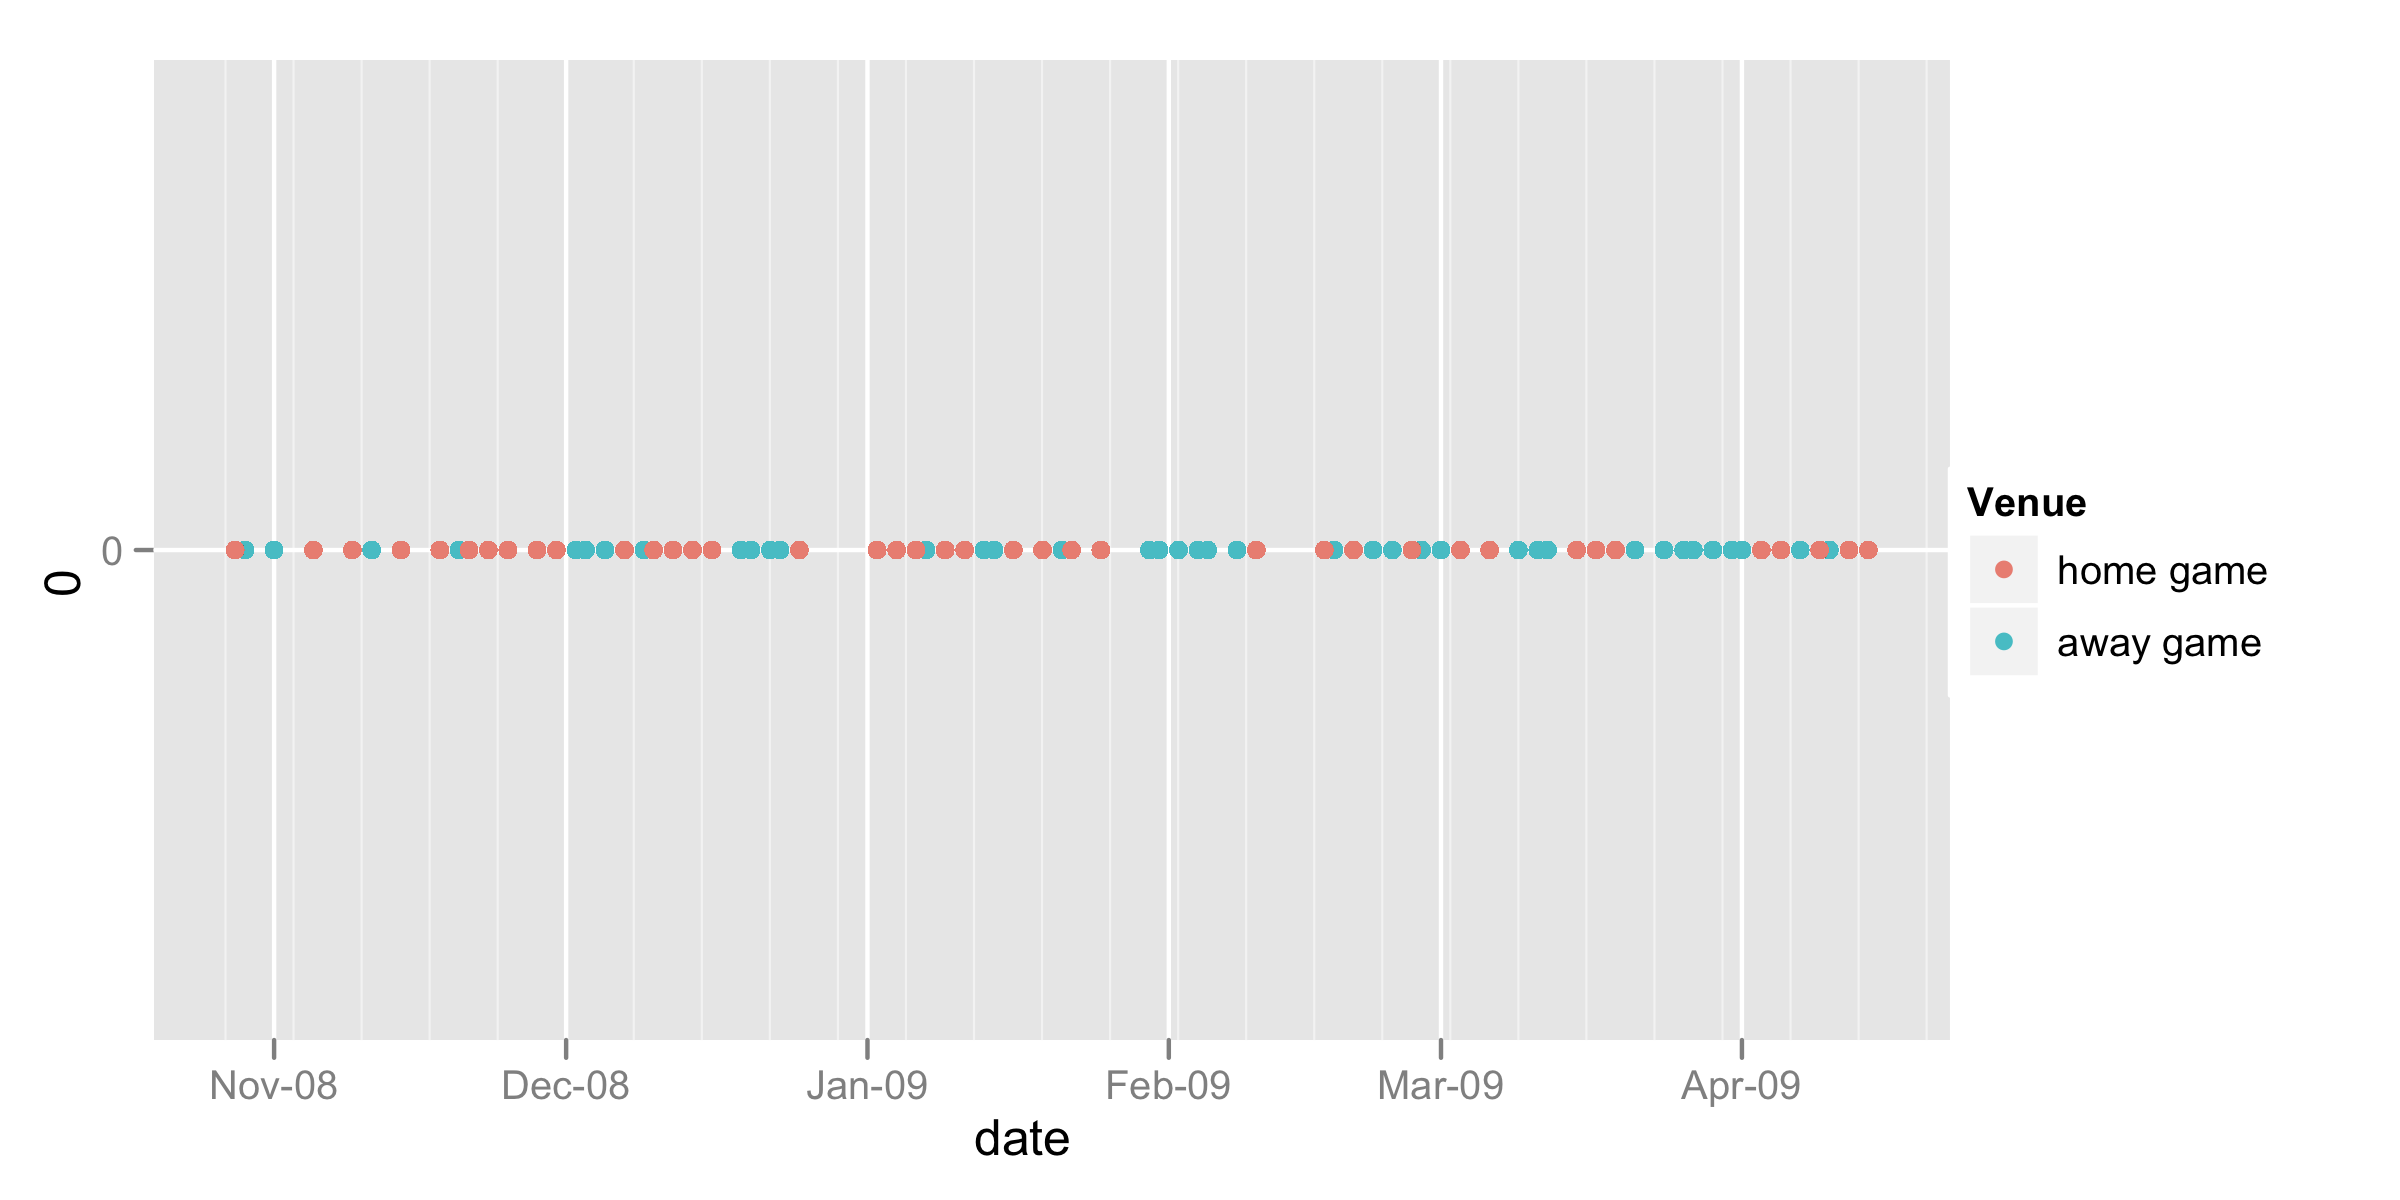
\includegraphics[width=\textwidth]{dates-points.png}        
  \caption{Dates of Lakers games for 2008-2009 season}
  \label{fig:games-date}
\end{figure}

Figure~\ref{fig:games-date} shows that games are played continuously throughout the season with a few short breaks. The frequency of games seems lower at the start of the season and games appear to be grouped into clusters of home games and away games. Notice the tick marks on the x axis; the labels and breaks are automatically generated by \code{pretty.date()}, which is in the \pkg{lubridate} package. 

Next we'll examine how Lakers games are distributed throughout the week.\\

\code{R> qplot(wday(date, label = T), data = lakers, geom = "histogram")}\\

\begin{figure}[htpb]
  \centering    
    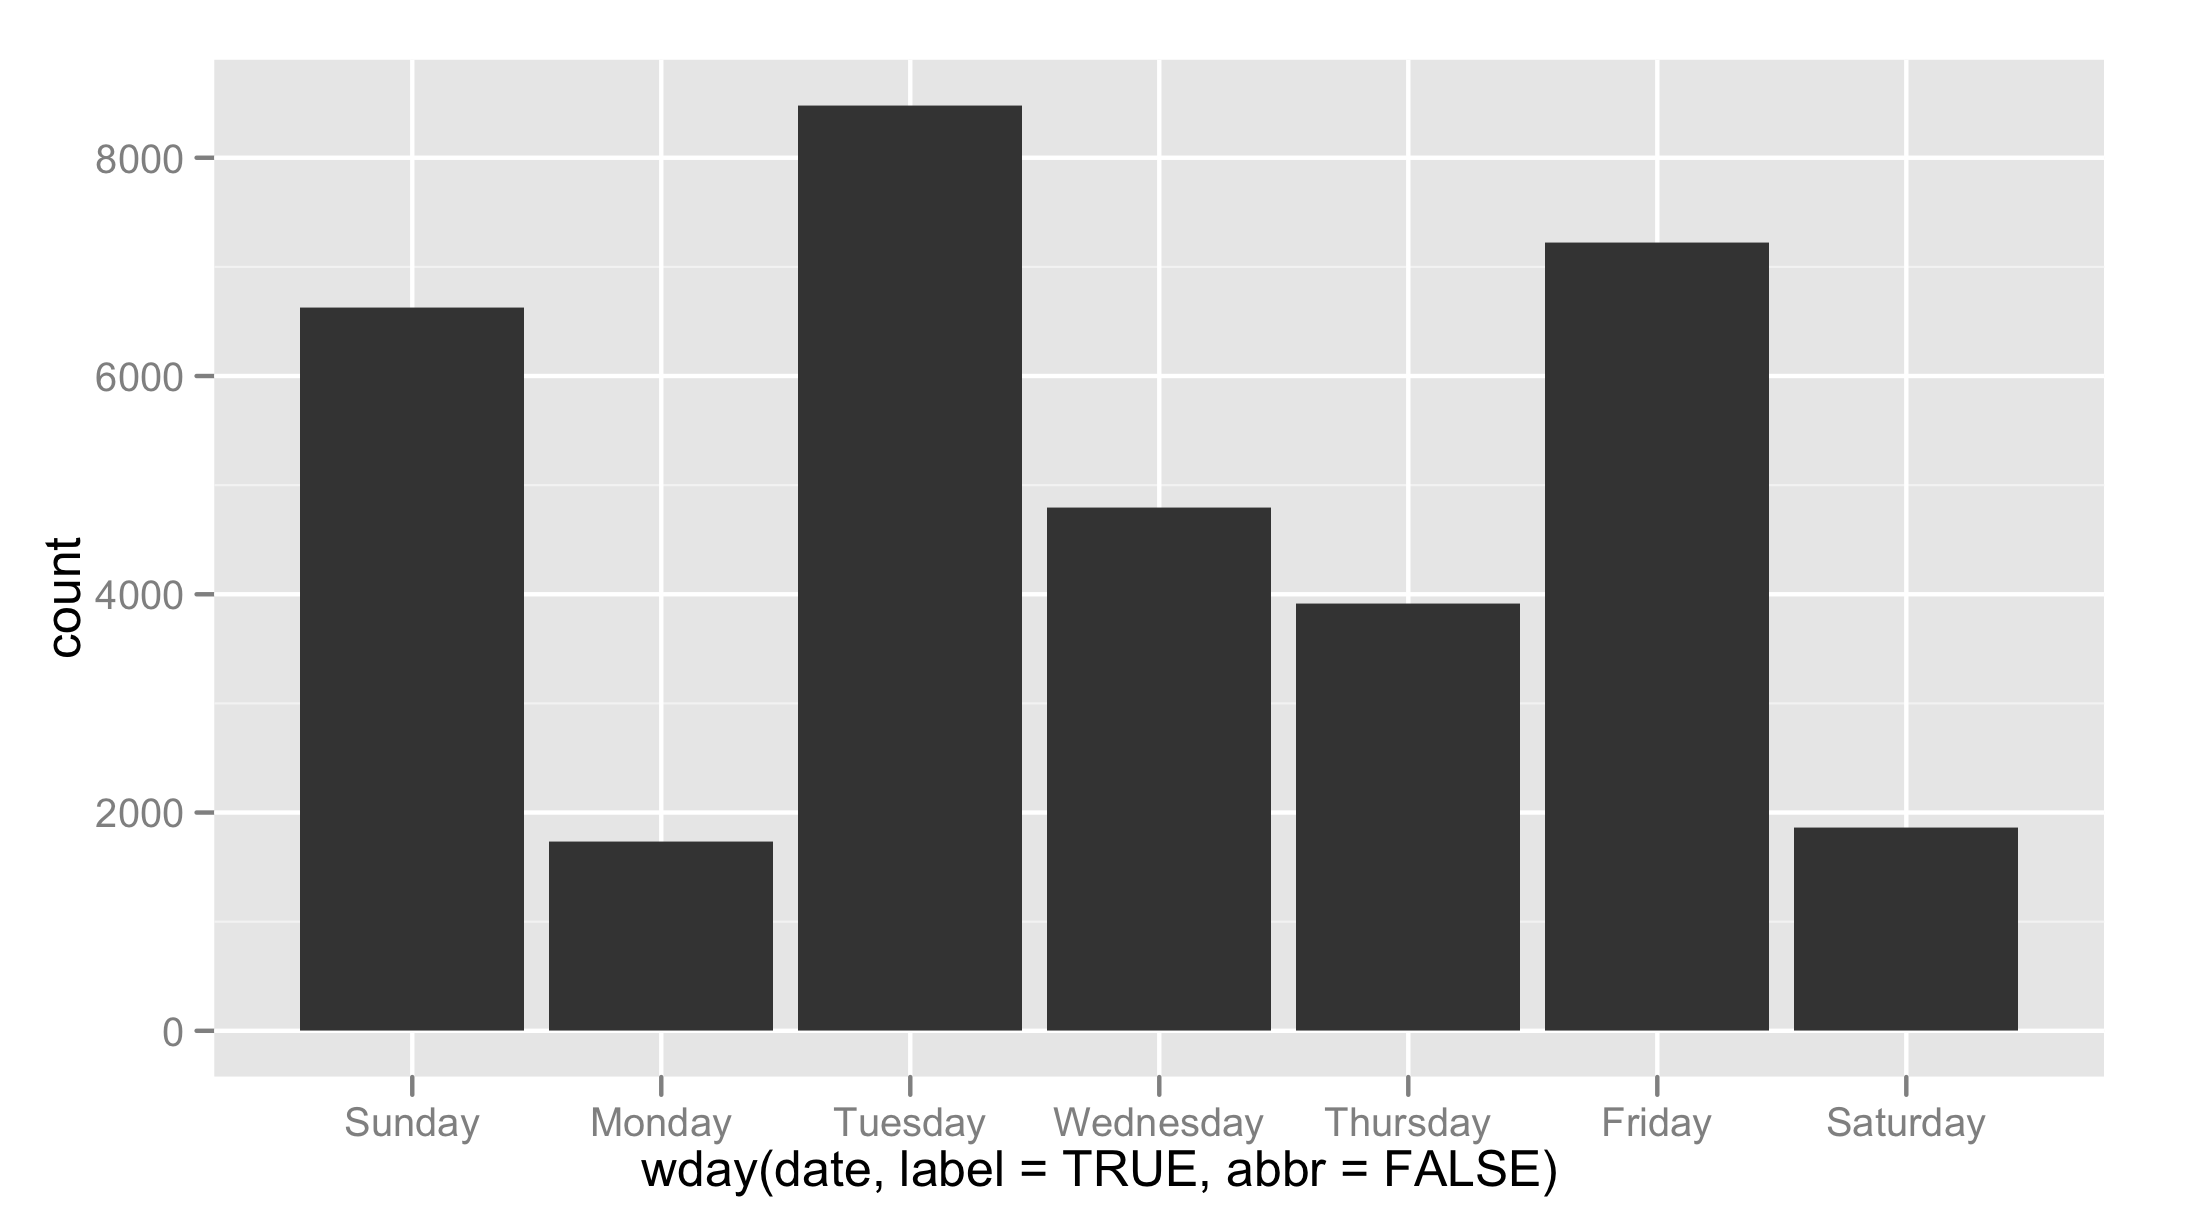
\includegraphics[width=\textwidth]{weekdays-histogram.png}     
  \caption{Number of games played per weekday}
  \label{fig:games-days}
\end{figure}


The frequency of basketball games appears to vary throughout the week, figure~\ref{fig:games-days}. Surprisingly, the highest number of games are played on Tuesdays.

Now let's look at the games themselves. In particular, let's look at the distribution of plays throughout the game. The \code{lakers} data set lists the time that appeared on the game clock for each play. These times begin at 12:00 at the beginning of each period and then count down to 00:00, which marks the end of the period. The first two digits refer to the number of minutes left in the period. The second two digits refer to the number of seconds.

The times have not been parsed as date-time data to \proglang{R}. In fact, it would be difficult to record the time data as a date-time object because the data is incomplete: a minutes and seconds element are not sufficient to identify a unique date-time. However, we can store the minutes and seconds information as a \emph{period} object, as defined in Section~\ref{sec:periods}, using the \code{ms()} parse function.\\

\code{R> lakers$time <- ms(lakers$time)}\\

Recall that periods have relative lengths. Since we'd like to compare times against each other, we should first convert our periods to \emph{durations}, which have exact lengths.\\

\code{R> lakers$time <- as.duration(lakers$time)}\\

This allows us to directly compare different durations. It would also allow us to determine exactly when each play occurred by adding the duration to the \emph{instant} the game began. (Unfortunately, the starting time for each game is not available in the data set). We can now subtract our time information from a duration of 12, 24, 36, or 48 minutes (depending on the period of play) to create a new duration that records exactly how far into the game each play occurred.\\

\code{lakers$time <- eminutes(12) * lakers$period - lakers$time}\\

Unfortunately, \pkg{ggplot2} does not support plotting durations, or difftimes, the class used by durations. To plot our data, we can extract the integer value of our durations, which will equal the number of seconds that occurred in each duration.\\

\code{R> qplot(as.integer(time), data = lakers, geom = "histogram", binwidth = 60)}\\

\begin{figure}[htpb]
  \centering
  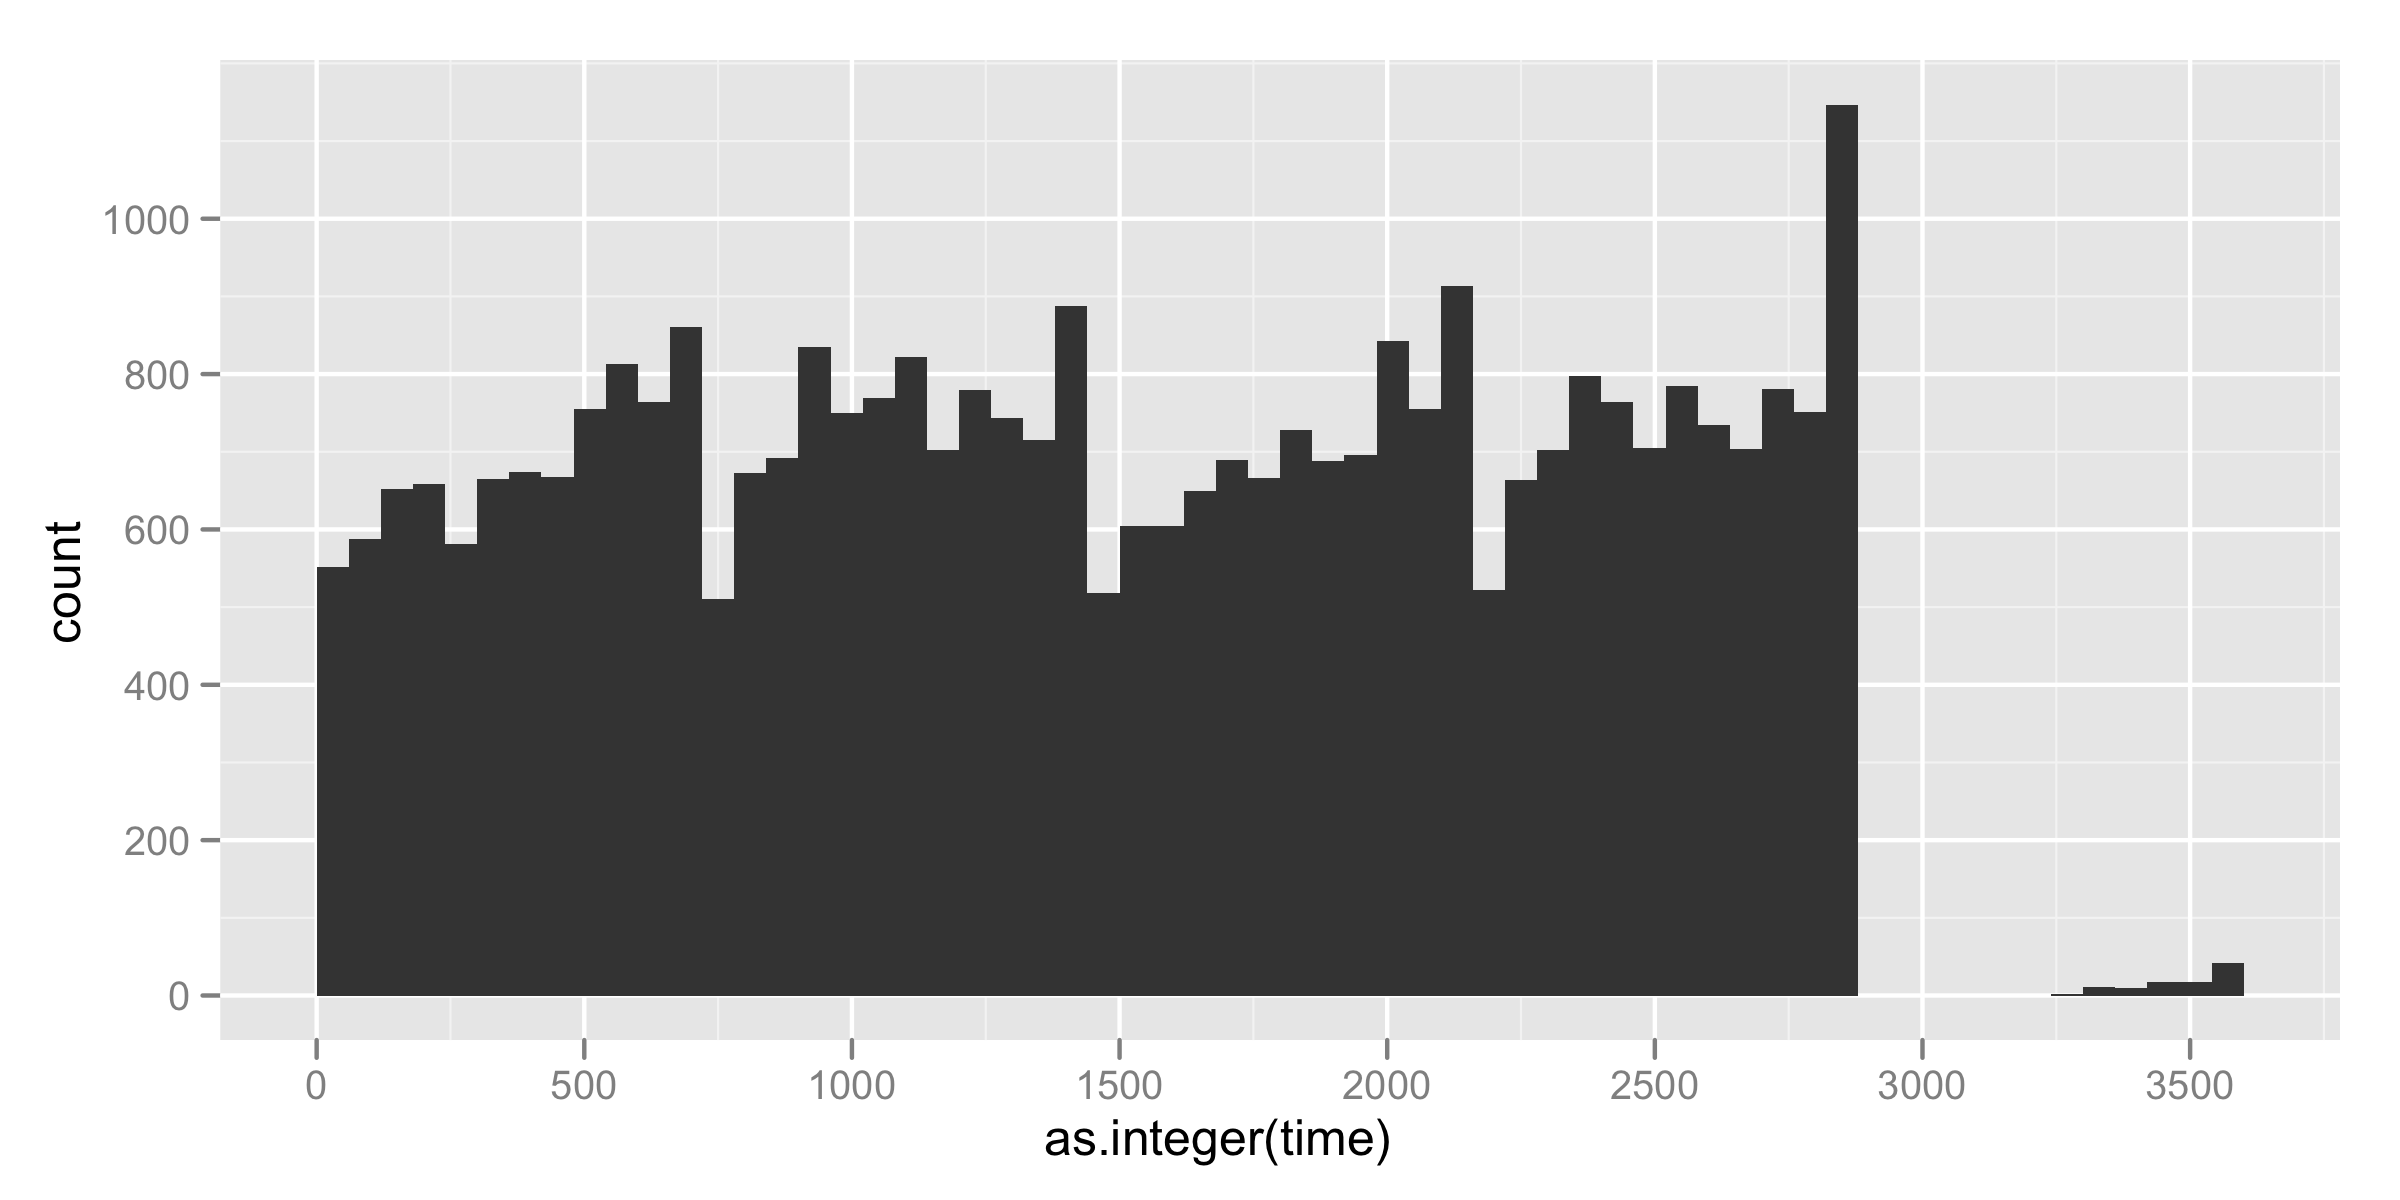
\includegraphics[width=\textwidth]{play-time-histogram.png}        
  \caption{Distribution of plays within game}
  \label{fig:plays}
\end{figure}

Alternatively, we can create date-times, which \pkg{ggplot2} does support, by adding each of our durations to the same starting instant. This creates a plot whose tick marks are determined by \code{pretty.date()}. This helper function recognizes the most intuitive binning and labeling of date-time data, which further enhances our graph.\\

\code{R> lakers$demo <- ymd("2008-01-01") + lakers$time}\\
\code{R> qplot(demo, data = lakers, geom = "histogram", binwidth = 60)}\\

\begin{figure}[htpb]
  \centering
  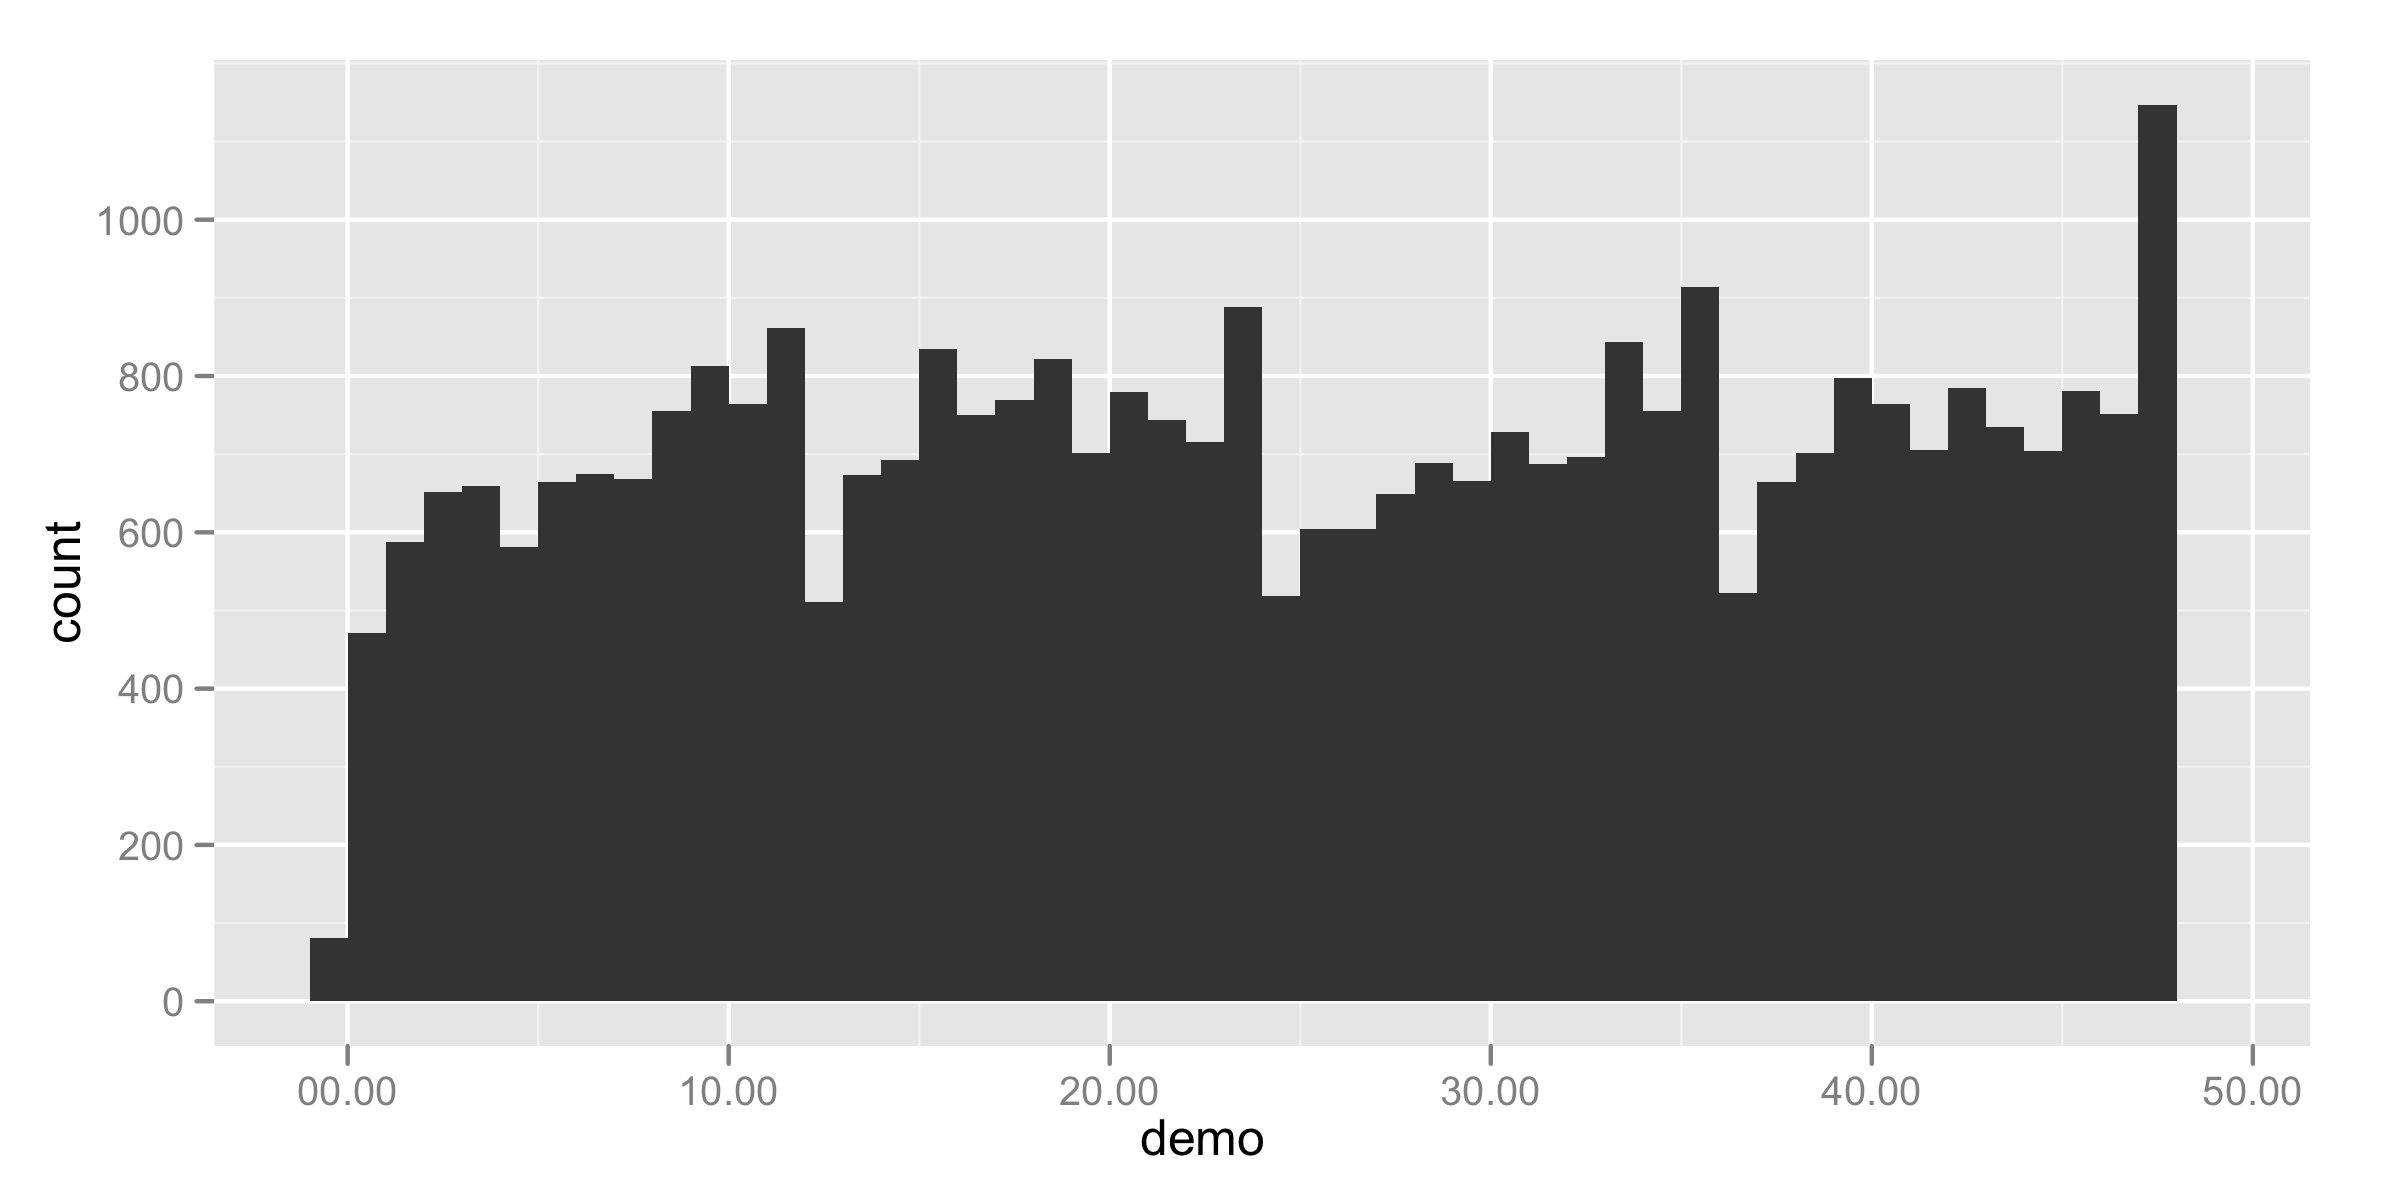
\includegraphics[width=\textwidth]{play-time-histogram2.png}        
  \caption{Distribution of plays within game}
  \label{fig:plays}
\end{figure}


We see that the number of plays peaks within each of the four periods and then plummets at the beginning of the next period, figure~\ref{fig:plays}. We also see a small number of plays that occur in overtime. Observations that occur after 48 minutes suggest games that were decided in overtime.

Now lets look more closely at just one basketball game: the first game of the season. This game was played on October 28, 2008. For this game, we can easily model the amounts of time that occurred between each shot attempt.\\

\code{R> game1 <- lakers[lakers$date == ymd("20081028"),]}\\
\code{R> attempts <- game1[game1$etype == "shot",]}\\

The waiting times between shots will be the time span that occurs between each shot attempt. Since we've recorded the time of each shot attempt as a duration (above), we can record the differences by subtracting the two durations. This automatically creates a new duration whose length is equal to the difference between the first two durations.\\

\code{R> attempts$wait <-  c(attempts$time[1], diff(attempts$time))}\\
\code{R> qplot(as.integer(wait), data = attempts, geom = "histogram", binwidth = 2)}\\

\begin{figure}[htpb]
  \centering
  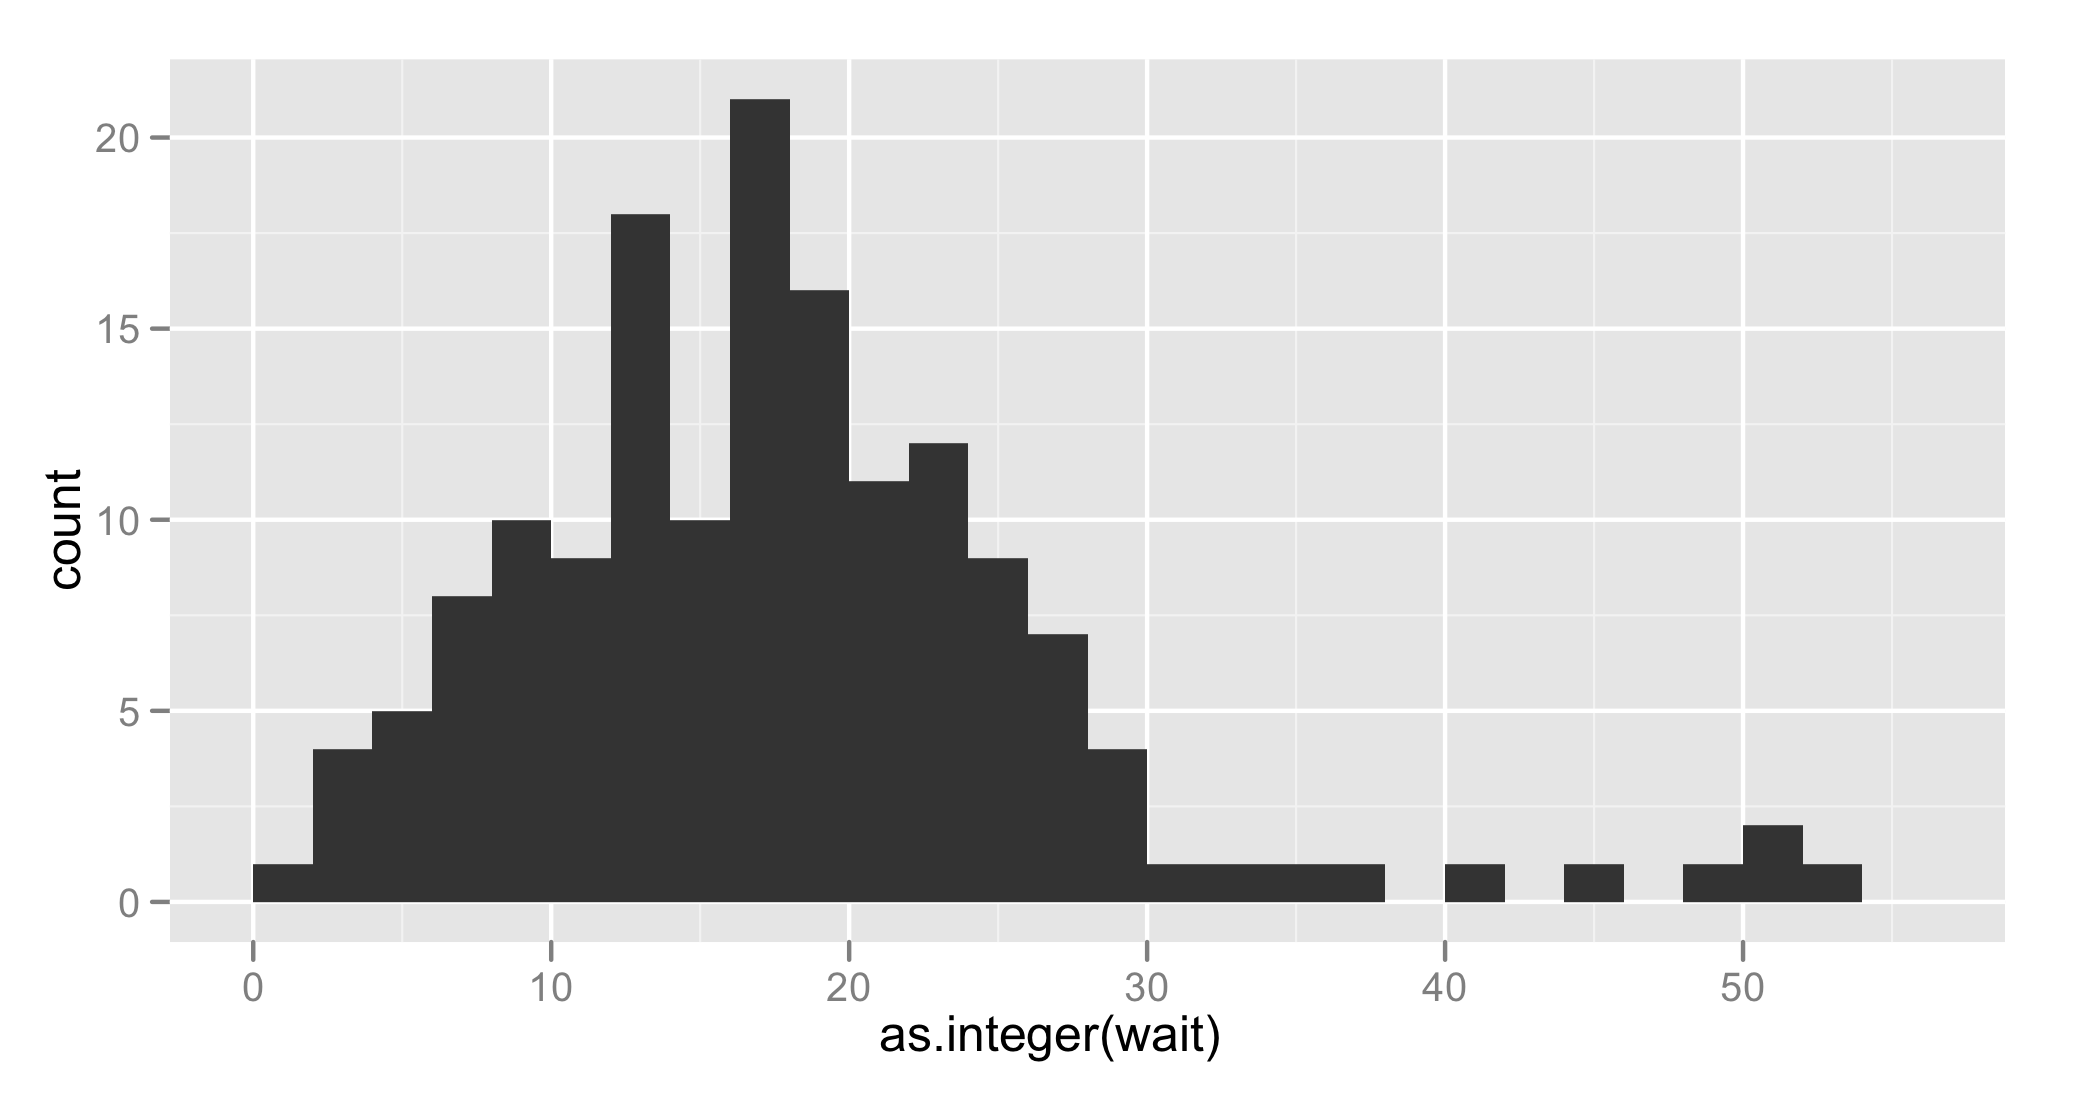
\includegraphics[width=\textwidth]{wait-histogram.png}        
  \caption{Distribution of wait times between shot attempts}
  \label{fig:waits}
\end{figure}

We plot this information in Figure~\ref{fig:waits}. We see that 30 seconds rarely go by without at least one shot attempt, but on occasion up to 60 seconds will pass without an attempt.

We can also examine changes in the score throughout the game. This reveals that the first game of the season was uneventful: the Lakers maintained a lead for the entire game, Figure~\ref{fig:scores}. Note: the necessary calculations are made simpler by the \code{ddply()} function from the \pkg{plyr} package, which \pkg{lubridate} automatically loads. \\

\code{R> game1_scores <- ddply(game1, "team", transform, score = cumsum(points))}\\
\code{R> game1_scores <- game1_scores[game1_scores$team != "OFF",]}\\
\code{R> qplot(ymd("2008-01-01") + time, score, data = game1_scores, geom = "line", colour = team)}\\

\begin{figure}[htpb]
  \centering
  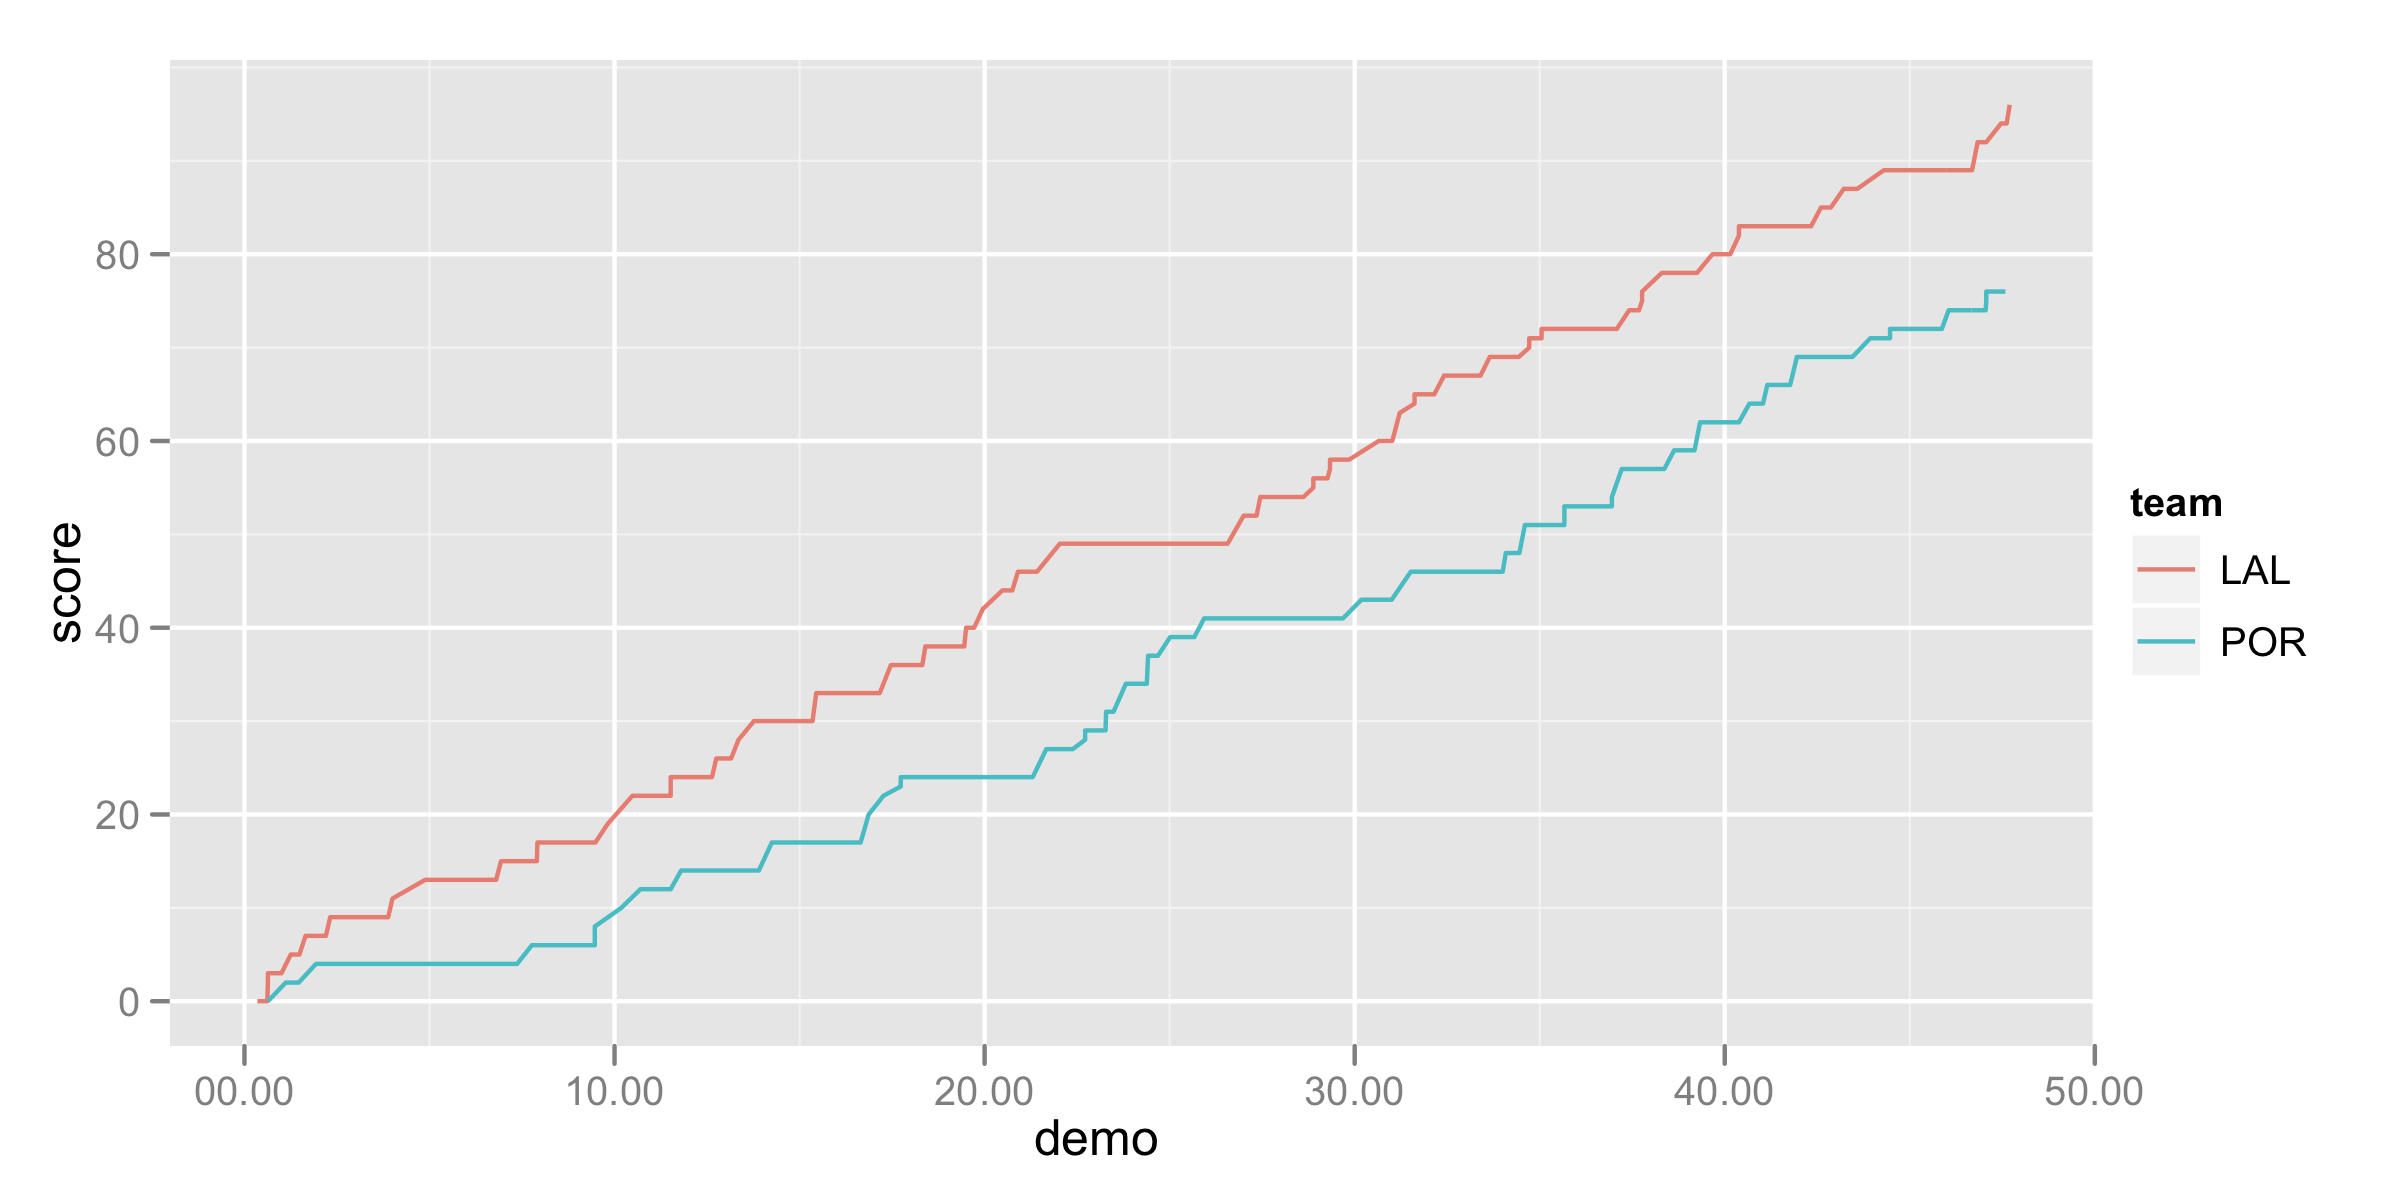
\includegraphics[width=\textwidth]{score-comparison.png}        
  \caption{Scores over time for first game of season}
  \label{fig:scores}
\end{figure}


\section{Conclusion}
Date-times create technical difficulties that other types of data do not. They must be specifically identified as date-time data, which can be difficult due to the overabundance of date-time classes. It can also be difficult to access and manipulate the individual pieces of data contained within a date time. Math with date-times is often appropriate, but must follow different rules than math with ordinal numbers. Finally, date related conventions such as daylight savings time and time zones make it difficult to compare and recognize different moments of time.

Base \proglang{R} handles many of these difficulties, but not all. Moreover, base \proglang{R}'s date-time methods are often complicated, confusing, and prone to change for different date-time classes. \pkg{lubridate} makes it to easier to work with date-time data in \proglang{R}. The package provides a set of standard methods for most common date-time classes. These methods make it simple to parse, manipulate, and perform math on date-time objects. By implementing the time concepts pioneered by the \proglang{java} based JODA time project, \pkg{lubridate} helps researchers perform precise calculations as well as model tricky time related processes. \pkg{lubridate} also makes it simple to switch date-times between time zones and to advantageously use or ignore daylight savings time.

Future work on the \pkg{lubridate} package will develop methods for handling partial dates and for modeling re-occuring events, such as stock market opening times, business days, or street cleaning hours. In particular, we hope to implement a method of defining reoccurring temporal patterns by extending the ideas created by the \proglang{Ruby} based \proglang{runt} project \citep{runts} to the \proglang{R} programming language.

\section*{Acknowledgements}
We'd like to thank the National Science Foundation. This work was supported by the NSF VIGRE Grant, number  DMS-0739420.


\bibliography{lubridate}


\end{document}
